\documentclass[a4paper,zihao=5,UTF8]{ctexart}
\usepackage[top=2.3cm,bottom=2cm,left=1.7cm,right=1.7cm]{geometry} 
\usepackage{amsmath, amssymb}
\usepackage{color}
\usepackage{hyperref} 
\usepackage{pythonhighlight}
\usepackage{listings}
\usepackage{mathrsfs} 
\usepackage{booktabs}
\usepackage{amsthm}
\usepackage{longtable} 
\usepackage{graphicx}
\usepackage{subfigure}
\usepackage{caption}
\usepackage{fontspec}
\usepackage{titlesec}
\usepackage{fancyhdr}
\usepackage{latexsym}
\usepackage{subfigure}
\usepackage{braket}
\usepackage{cite}
\usepackage[version=4]{mhchem}

\CTEXsetup[format={\Large\bfseries}]{section}
\def\d{\mathrm{d}}
\def\e{\mathrm{e}}
\def\i{\mathrm{i}}
\def\dps{\displaystyle}
\newcommand{\mr}[1]{\mathrm{#1}}
\newcommand{\mb}[1]{\mathbf{#1}}
\newcommand{\dv}[2]{\frac{\d{#1}}{\d{#2}}}
\newcommand{\pdv}[2]{\frac{\partial{#1}}{\partial{#2}}}
\def\degree{$^{\circ}$}
\def\celsius{^{\circ}\mr{C}}
\title{\textbf{实验四 1,3,5-三甲苯三羰基钼的制备与表征\cite{inorganic_chemistry_1}}}
\author{王崇斌\;1800011716}
\makeatletter
\makeatother
\begin{document}
	\pagestyle{fancy}
	\pagestyle{fancy}
    \lhead{无机化学实验}
	\chead{}
	\rhead{\today}
	\maketitle
    \thispagestyle{fancy}
	\section{实验原理}
	\subsection{金属羰基化合物}
	CO是一种中性配体,其能与很多低价态(零价态)的过渡金属形成丰富稳定的配合物,它们的
	结构性质与催化性能引起了人们的较大兴趣。这里简要介绍一下金属羰基配合物的成键特点
	,解释为什么CO可以与过渡金属形成比较稳定的配合物(这种配合物与传统的正负电中心形成的
	配合物有着明显不同)。
	\par 
	CO是一个典型的$\sigma$给体与$\pi$受体,其分子轨道能级如图(\ref{CO_MO})所示,
	\begin{figure}[htbp]
		\centering
		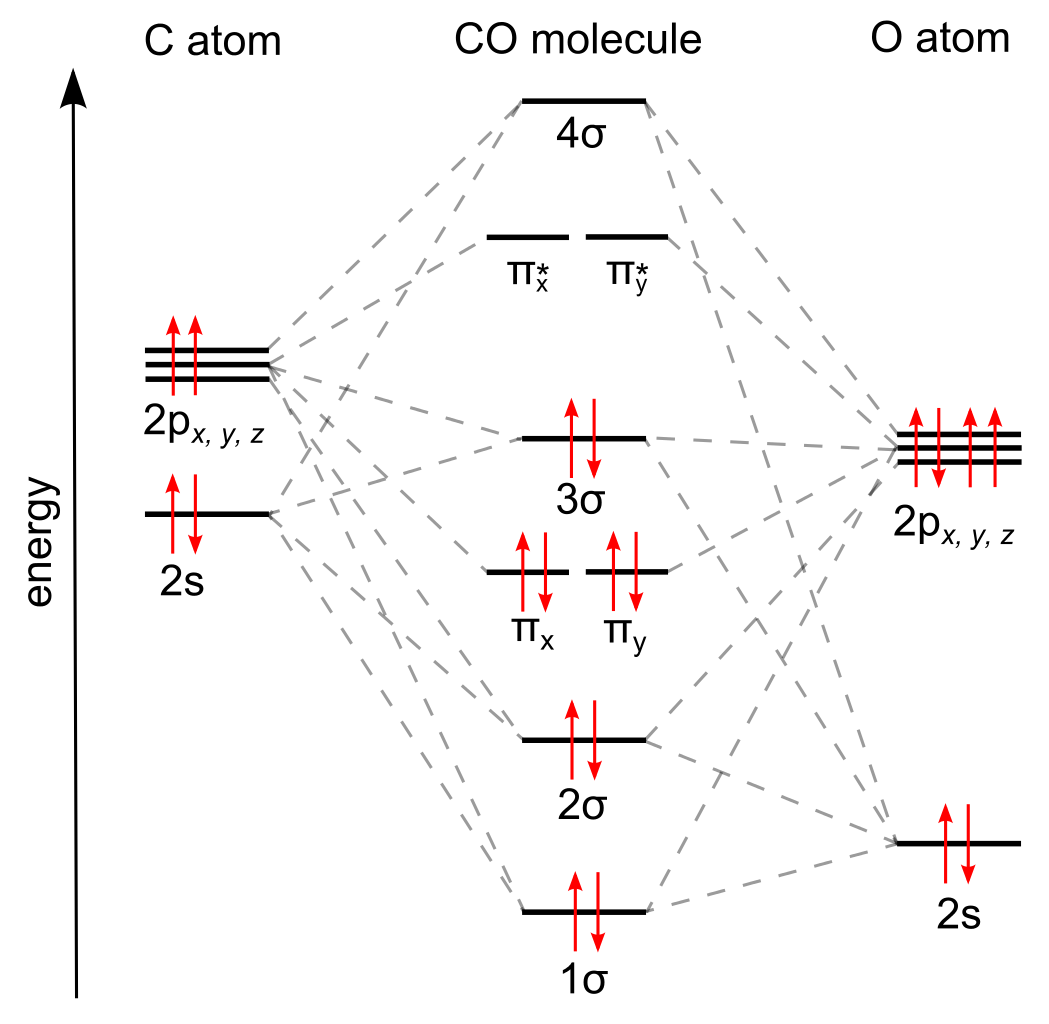
\includegraphics[scale=0.2]{MO_CO.png}
		\caption{CO分子轨道能级图}
		\label{CO_MO}
	\end{figure}
	可以看到CO的HOMO为主要集中在C原子上的$3\sigma$轨道,LUMO为主要集中在C原子上的$\pi^*$
	轨道,这两个轨道的示意图可以参考图(\ref{CO_HOMO_LUMO})。
	\begin{figure}[htbp]
		\centering 
		\begin{tabular}{cc}
		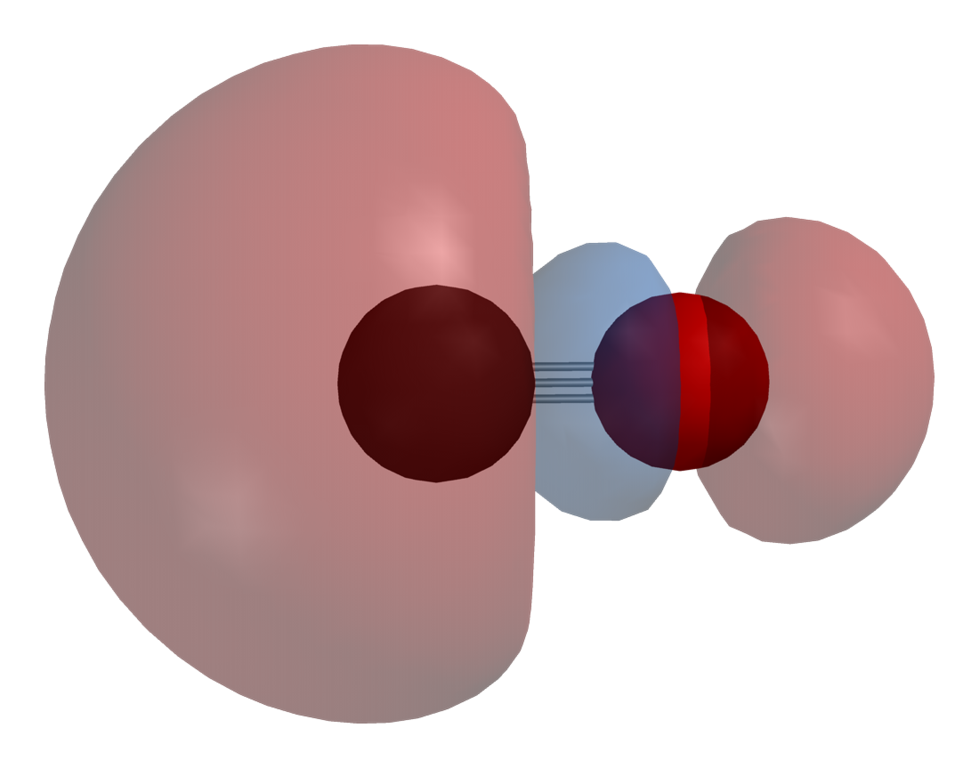
\includegraphics[scale=0.1]{Carbon-monoxide-HOMO-phase-3D-balls.png}
		&
		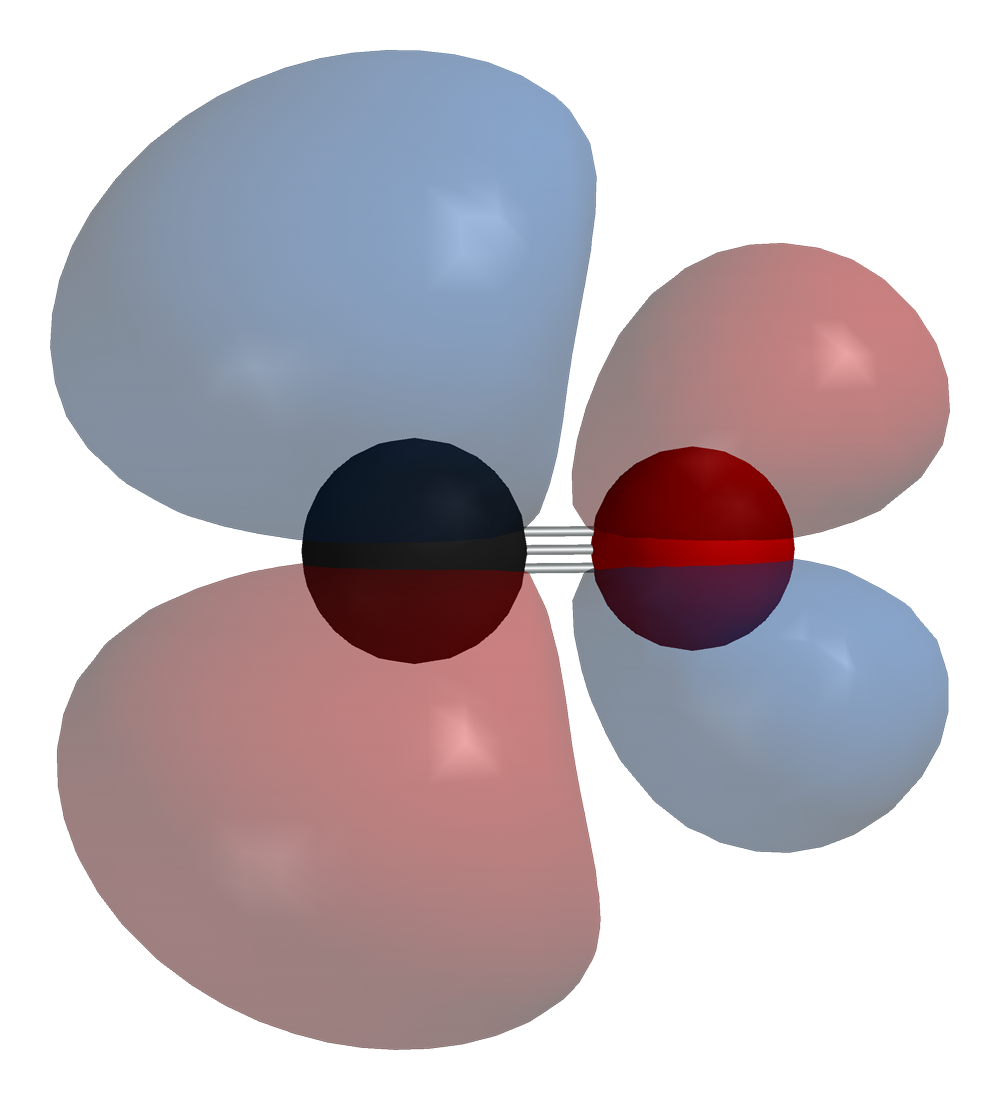
\includegraphics[scale=0.1]{Carbon-monoxide-LUMO-phase-3D-balls.png}
		\end{tabular}
		\caption{CO的前线轨道示意图}
		\label{CO_HOMO_LUMO}
	\end{figure}
	当CO与金属成键时,$3\sigma$轨道会与金属具有相同对称性的\textbf{空}轨道(一般是d,s,p混合而成)
	形成$\sigma$配位键,金属\textbf{填充电子}的d轨道会与CO空的$\pi^*$轨道形成反馈$\pi$键,
	形成这样的键要求金属有充足的d电子,这解释了CO倾向于与低价金属配位;由于d电子
	填入CO的$\pi^*$轨道,降低了金属的电子密度,使整个配合物更稳定,同时削弱了C-O键,
	使得其振动频率下降,这可以从红外光谱的数据得到证实。图\ref{M-CO}示意了CO与金属的成键过程。
	\begin{figure}
		\centering 
		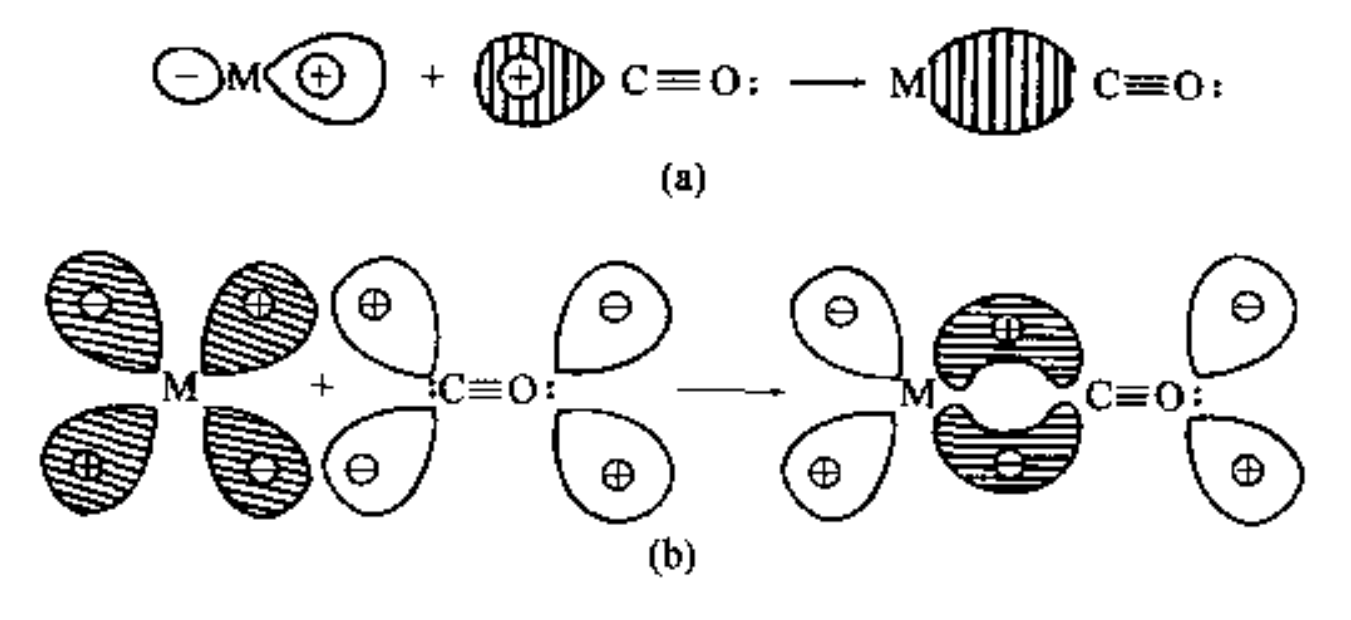
\includegraphics[scale=0.25]{M_CO.png}
		\caption{M-CO之间$\sigma-\pi$配位键示意图\cite{comprehensive_inorganic_chemistry}}
		\label{M-CO}
	\end{figure}
	\subsection{金属环多烯配合物}
	早在蔡斯盐(\ce{K[Pt(C_2H_4)Cl_3]*x H_2O})中,人们就认识到烯烃能够与金属配位,但是当时的人们并没有正确认识
	烯烃与金属配位时的成键方式。第一个苯的$\pi$配合物二苯铬直到1955年才确定其结构为类似二茂铁的夹心型配合物,
	从苯的电子结构上看,它可以看作3个烯烃配位,提供6个电子。但是实验数据表明,
	配体中苯的碳碳键依然等长,并非形成三个定域的烯烃配位。应将苯配体视为一个整体,
	利用分子轨道理论(考虑配体的$\pi$轨道与金属的d轨道相互作用)解释它与金属的配位方式和光谱特性。
    \section{实验过程}
    实验地点:北京大学化学院D区3楼第一教学实验室2号实验台
	\par 
	实验时间:2021年4月17日(星期五)
	\subsection{制备\ce{[1,3,5-C_6H_3(CH_3)Mo(CO)_3]}}
	在20ml支管圆底烧瓶中加入200mg(206mg)\ce{Mo(CO)_6}、2ml均三甲苯,按照图(\ref{shiyanzhuangzhi})
	\begin{figure}[htbp]
		\centering
		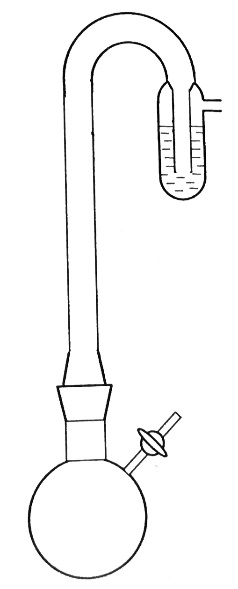
\includegraphics[scale=0.8]{shiyanzhuangzhi.png}
		\caption{实验反应装置}
		\label{shiyanzhuangzhi}
	\end{figure}
	搭好反应装置。
	\par
	由于\ce{Mo(CO)_6}在温度较高时会与空气中的氧作用,因此反应需在惰性气氛中进行。
	把烧瓶的支管接通氮气源,开始时用氮气以较快速度冲洗体系(以油封处气泡成串为宜,不宜过快)
	,5分钟后开始缓慢加热升温,继续通5分钟氮气(此时速度应稍慢,气泡冒出速率为1个每秒为宜)
	。每隔一段时间提高一次加热电压(每次10 ~ 20 V),开始时可以观察到\ce{Mo(CO)_6}升华
	并且在烧瓶瓶颈处凝华形成白色半透明状晶体,晶体不断增多(个人推测这是实验产率低的一个
	重要原因),随着加热进行,溶液逐渐变为淡黄色,当电压达到100V时,溶液开始回流,溶液的黄色不断加深
	。可以看到
	均三甲苯不断地将烧瓶瓶颈上的\ce{Mo(CO)_6}冲洗下来,\ce{Mo(CO)_6}继续在温度低的地方凝华
	,聚集在冷凝管中。约30分钟后,烧瓶内壁产生一层钼膜,溶液颜色不再加深,此时停止加热,
	从砂浴中取出烧瓶,缓缓通氮气以避免油封倒吸。静置冷却。
	\par
	当反应器冷却至室温,关闭\ce{N_2}并拆散装置,将烧瓶中的溶液用滴管转移至小锥形瓶中
	(注意锥形瓶容易倒,放在烧杯中比较稳妥),向其中加入8ml石油醚,观察到有黄色沉淀生成
	。静置,用滴管移去大部分上清液,将剩下的沉淀用滴管转移至玻璃滴管柱内,挤去母液保留沉淀,
	用1ml左右石油醚洗涤沉淀,理想的沉淀为淡黄色,实验中得到的沉淀为绿色且其中混有黑色杂质
	(单质Mo)。
	\par
	在滴管柱内分批加入总量约1.5ml的二氯甲烷,充分溶解滴管柱内的产物,将滤液收集在小锥形瓶
	中,过滤时注意观察滴管内滤液的颜色,如果颜色明显变淡或者滤液无色就应该立即停止加入
	二氯甲烷
	\footnote{
		在实验过程中实验者加入了1.5ml二氯甲烷但是滤液依然是明显的黄色,实验者害怕
		加入更多的二氯甲烷会影响下一步晶体析出因而没有继续加入二氯甲烷。但是通过
		后续对滴管柱内二氯甲烷滤液中加入石油醚后又较多沉淀可以判断此步骤中损失了
		较多的产物。
	}
	。在滤液中加入5ml石油醚,可以观察到有大量淡黄色沉淀析出,用砂芯漏斗抽滤,结晶
	使用2ml石油醚分两次淋洗,抽干,母液在室温下用油泵减压浓缩,再得到一些产品。
	获得干燥的黄色粉末状产物40mg,产率17\%。
	\subsection{测定\ce{[1,3,5-C_6H_3(CH_3)Mo(CO)_3]}的红外光谱}
	将上述制得的\ce{[1,3,5-C_6H_3(CH_3)Mo(CO)_3]}约1mg(用小药匙取一点,不用称量)
	与KBr约300mg用玛瑙研钵研磨均匀,压片。在红外光谱仪上记录产物的红外光谱
	(400-4000 $\mr{cm}^{-1}$)。配体的红外光谱不做,相应图谱参考教材附图。
	\subsection{测定\ce{1,3,5-C_6H_3(CH_3)_3}与\ce{[1,3,5-C_6H_3(CH_3)Mo(CO)_3]}的核磁共振氢谱}
	本部分由于实验时间问题不做,谱图参考讲义。
	\subsection{测定\ce{[1,3,5-C_6H_3(CH_3)Mo(CO)_3]}的质谱}
	本部分由于实验时间问题不做,谱图参考讲义。
    \section{结果与讨论}
	\subsection{关于产品收率}
	前文中已经给出了产率为17\%(理论产量为232mg),个人认为最影响产率的两个因素是
	\ce{Mo(CO)_6}的升华(通过实验观察,升华的量很可观,可以占到称量反应物的30\%
	以上)与反应中\ce{Mo(CO)_6}的分解(这就要求保持无氧环境、控制温度)。还有一个
	可以从操作中改进的地方,之前也提到过,在用二氯甲烷溶解产物的过程中,应该加入足够的
	溶剂直到滤液颜色明显变浅,而不能照搬实验讲义上的量。

	\subsection{关于红外光谱}
	实验中产物的红外光谱如图(\ref{IR}所示
	\begin{figure}[htbp]
		\centering 
		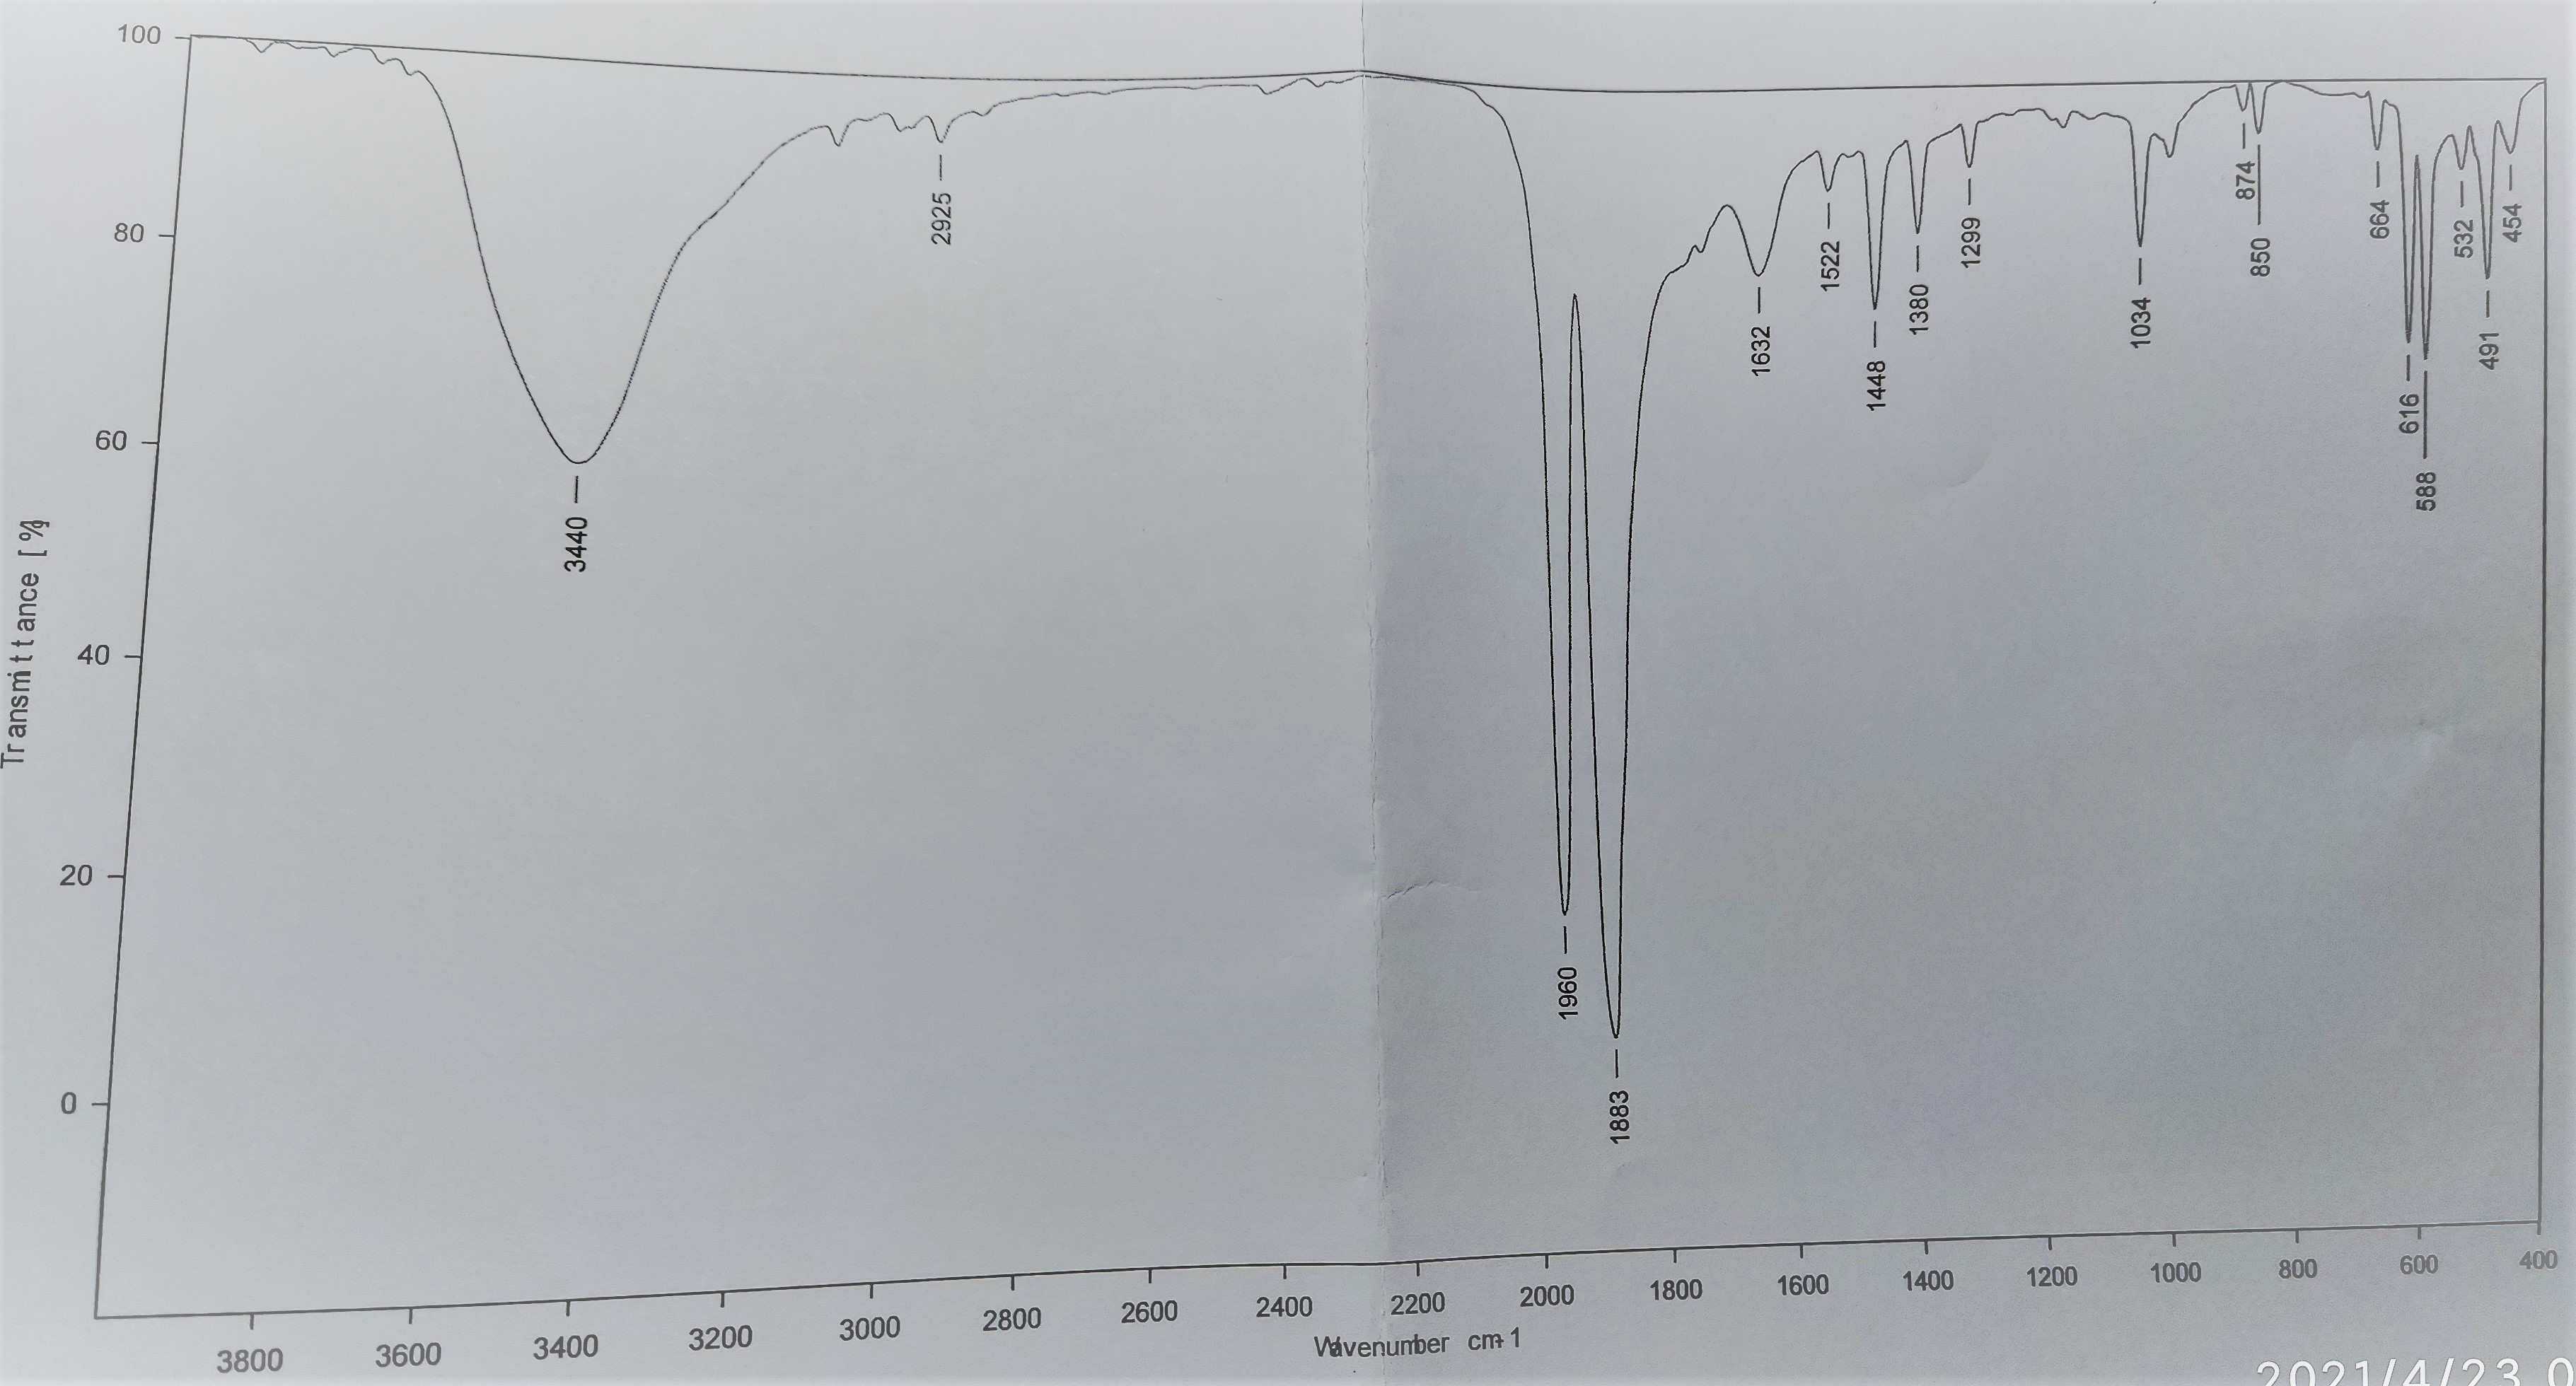
\includegraphics[scale=0.10]{IR.jpg}
		\caption{\ce{[1,3,5-C_6H_3(CH_3)Mo(CO)_3]}的红外光谱}
		\label{IR}
	\end{figure}
	,与讲义上反应物的IR谱图对比结合IR相关知识可知:
	\par 
	对于\ce{Mo(CO)_6},3438$\mr{cm}^{-1}$附近的宽峰不知来源。1976$\mr{cm}^{-1}$
	附近的尖锐峰是C-O的伸缩振动,592$\mr{cm}^{-1}$附近尖锐峰猜测是Mo-C的弯曲振动。
	\par 
	对于均三甲苯,关注几个尖锐的峰(尖锐的峰一定对应对称性高、比较单纯的振动模式
	),3000$\mr{cm}^{-1}$附近的是芳环上C-H键的伸缩振动,
	2900$\mr{cm}^{-1}$附近是甲基上C-H键的伸缩振动,1472$\mr{cm}^{-1}$
	应该对应甲基不对称面内摇摆振动、1376$\mr{cm}^{-1}$应该对应甲基的剪式振动。
	1608$\mr{cm}^{-1}$处极其尖锐的峰应该对应苯环C-C键的伸缩振动,835$\mr{cm}^{-1}$
	与687$\mr{cm}^{-1}$应该对应了苯环上C-H键的面外弯曲振动。
	\par 
	对于产物,3440$\mr{cm}^{-1}$附近的宽峰应该对应于甲基和苯环上C-H键的伸缩振动。
	1960$\mr{cm}^{-1}$与1883$\mr{cm}^{-1}$处对应了C-O的伸缩振动,与\ce{Mo(CO)_6}
	中的数据比较可知,振动频率减小,这说明金属原子更加富电子(苯环提供了电子),削弱了
	羰基中的键。1632$\mr{cm}^{-1}$对应苯环C-C键的伸缩振动,1448$\mr{cm}^{-1}$,1380$\mr{cm}^{-1}$
	对应了甲基的面内摇摆和剪式振动,这些与配体中的光谱数据没有明显差别。
	\subsection{关于NMR}
	观察讲义中两种反应物的谱图,根据峰面积积分容易指认,均三甲苯位于6.79ppm处为苯环氢,
	2.27ppm处为甲基氢,均与一般芳香有机化合物中峰位置相似。而在产物中,甲基氢的峰
	未发生明显位移,仍位于2.27ppm处,说明在配位过程中甲基氢的化学环境改变很小,
	不存在抓氢键等金属有机化合物中时常出现的特殊键型。而苯环氢的化学位移产生了明显改变,
	移动至5.24ppm处,这说明在配位过程中,苯环的π电子流向金属,电子环流减弱,
	导致对芳氢的去屏蔽效应减弱,使得苯环上氢的化学位移向高场移动,这与IR中C-O的伸缩振动
	频率降低所反映出来的金属电子密度增加互相印证。
	\subsection{关于质谱}
	本次实验产物的化学式为\ce{MoC_{12}H_{12}O_3},其中需要考虑的主要是C的同位素:C-12,98.89\%;
	C-13,1.11\%;和Mo的同位素:Mo-92,15.86\%;Mo-94,9.12\%;Mo-95,15.70\%;Mo-96,
	16.50\%;Mo-97,9.45\%;Mo-98,23.75\%;Mo-100,9.62\%。
	\par 
	由于C-13的丰度较低,只考虑全为C-12($0.988912^{12} = 87.46\%$)和一个C-13的情况($C_{12}^{1}\times 0.111 = 0.133$),
	不考虑多个C-13的情况。那么可以组合出质谱图中给出的各种信号,列于表中,其中每一个产物出现的概率
	可以由Mo同位素出现的概率和C同位素出现的概率相乘而计算出,这个有可能可以解释谱图中的强度信息。
	\begin{table}[htbp]
		\centering
		\caption{产物的同位素组成}
		\label{iso}
		\begin{tabular}{ccc}
			\toprule
			分子量 & C-13数量 & Mo同位素 \\
			\midrule
			296	& 0 & 92 \\
			297	& 1	& 92 \\
			298	& 0	& 94 \\
			299	& 1/0 & 94/95 \\
			300	& 1/0 & 95/96 \\
			301	& 1/0 & 96/97 \\
			302 & 1/0 & 97/98 \\
			303	& 1 & 98 \\
			304	& 0 & 100 \\
			305	& 1	& 100\\
			\bottomrule
		\end{tabular}
	\end{table}
    \bibliographystyle{plain}
	\bibliography{ref}
\end{document}